\documentclass[11pt]{article}

\usepackage[margin=1in]{geometry}
\usepackage{amsmath,amsthm,amsfonts}
\usepackage[utf8]{inputenc}
\usepackage{amssymb}
\usepackage[mathscr]{eucal}
\usepackage{graphicx}
\usepackage{listings}
\usepackage{titlesec}
\usepackage{tikz}
\usepackage{xcolor}
\usepackage[OT1]{fontenc}
\usepackage{physics}
\usepackage{xpatch}

\usetikzlibrary{graphs}
\usetikzlibrary{graphs.standard}

\setlength\parindent{0pt}

\newtheoremstyle{dotless}{}{.5\topsep}{\itshape}{}{\bfseries}{}{ }{}

\newtheoremstyle{dotles}{}{}{\upshape}{}{\bfseries}{}{ }{}

\theoremstyle{definition}
\newtheorem*{defin}{DEF}

\theoremstyle{dotles}
\newtheorem{innercustomex}{EX}
\newenvironment{exercise}[1]
  {\renewcommand\theinnercustomex{#1}\innercustomex}
  {\endinnercustomex}

\theoremstyle{dotless}
\newtheorem{proposition}{PROP}[section]

\theoremstyle{remark}
\newtheorem{remark}{Remark}
\newtheorem{example}{Example}

\usepackage{hyperref}
\hypersetup{colorlinks=false}

\titleformat{\section}
{\normalfont\Large\bfseries}{\S\thesection.}{1em}{}



\begin{document}

\section{Fundamental Concepts}

\begin{proposition}
An edge is a cut-edge if and only if it belongs to no cycle.
\end{proposition}

\begin{remark}
Every $u,v$-walk contains a $u,v$-path, and every closed odd walk contains an odd cycle. These can be proved by induction. But an even closed walk may not contain a cycle. Indeed, for
\[\begin{tikzpicture}
\filldraw(-2,0)circle(2pt)node[align=left,below]{$a$}--node[above]{$r$}++(2,0)circle(2pt)node[align=center,below]{$x$}--node[above]{$t$}++(2,0)(2,0)circle(2pt)node[align=right,below]{$c$};
\filldraw(0,2)circle(2pt)node[right]{$b$}--node[left]{$s$}(0,0);
\end{tikzpicture},\]
the even closed walks $a,r,x,s,b,s,x,r,a$ and $a,r,x,s,b,s,x,t,c,t,x,r,a$ do not contain a cycle.
\end{remark}

\begin{proposition}[König {[1936]}]
A graph is bipartite if and only if it has no odd cycle.
\end{proposition}

\begin{proposition}
The complete graph $K_n$ can be expressed as the union of $k$ bipartite graphs if and only if $n\leq2^k$.
\end{proposition}

\begin{proposition}
A graph is Eulerian if and only if all vertices are even and it has at most one nontrivial component.
\end{proposition}

\begin{proposition}
The minimum number of trails decomposing a connected nontrivial graph with exactly $2k$ odd vertices is $\max\{k,1\}$.
\end{proposition}

\begin{proposition}[Degree-Sum Formula]
\[\sum_{v\in V(G)}d(v)=2e(G).\]
\end{proposition}

\begin{proposition}
For a simple graph with vertices $v_1,v_2,\cdots,v_n$ and $n\geq3$, $(n-2)e(G)=\sum_ie(G-v_i)$ and $e(G)=(n-2)(d(v_i)+e(G-v_i))$.
\end{proposition}

\begin{proposition}[Mantel [{1907]}]
$K_3$-free simple graph of order 3 has at most $\left\lfloor n^2/4\right\rfloor$ edges.
\end{proposition}



\newpage\appendix
\section*{Definition Page}
A \textbf{graph} $G$ is a triple $(V(G),E(G),f)$ where $V(G)$ is the vertex set, $E(G)$ is the edge set, and $f$ associates two vertices with each edge. $n(G)=\abs{V(G)}$ is the \textbf{order} of $G$, and $e(G)=\abs{E(G)}$ is the \textbf{size} of $G$. A \textbf{subgraph} $H$ of $G$ is a graph such that $V(H)\subseteq V(G)$, $E(H)\subseteq E(G)$, and $f_H=f$. A \textbf{decomposition} of a graph is a list of subgraphs such that each edge appears exactly once in each subgraph. A \textbf{disjoint union} of graphs is the union of graphs with distinct vertex sets.\medbreak
Endpoints are \textbf{adjacent} if they are endpoints of a same edge. A \textbf{clique} in a graph is a set of pairwise adjacent vertices. An \textbf{independent set} in a graph is a set of pairwise non-adjacent vertices. A graph $G$ is \textbf{$k$-partite} if $V(G)$ can be expressed as the union of $k$ independent sets (\textbf{partite sets}). An \textbf{$X,Y$-bigraph} is a 2-partite graph with partite sets $X$ and $Y$. The \textbf{chromatic number} $\chi(G)$ of $G$ is the minimum number of colors needed to label the vertices so that adjacent vertices receive different colors. Vertex $v$ and edge $e$ are \textbf{incident} if $v$ is the endpoint of $e$. The \textbf{degree} $d(v)$ of $v$ is the number of incident edges. \textbf{Isolated vertex} has vertex degree 0. A graph is \textbf{even} or \textbf{odd} if all vertices are even or odd. A graph is \textbf{$k$-regular} if $\Delta(G)=\delta(G)=k$ where $\Delta(G)$ and $\delta(G)$ are maximum and minimum degrees of $G$.\medbreak
A graph is \textbf{simple} if it has no loops or edges having the same pair of endpoints. The \textbf{complement} $\overline{G}$ of simple graph $G$ is the simple graph with vertex set $V(G)$ and $uv\in E(\overline{G})$ if and only if $uv\not\in E(G)$. A \textbf{complete} graph $K_n$ is a simple graph with $n$ pairwise adjacent vertices. A \textbf{biclique} $K_{r,s}$ is a simple bipartite graph such that two vertices are adjacent if and only if they are in different partite sets of orders $r$ and $s$.\medbreak
Let $G$ be a loopless graph, $V(G)=\{v_1,v_2\cdots,v_n\}$, and $E(G)=\{e_1,e_2\cdots,e_m\}$. The \textbf{adjacency matrix} $A(G)$ of $G$ is the $n$-by-$n$ matrix in which $a_{ij}$ is the number of edges in $G$ with endpoints $\{v_i,v_j\}$. The \textbf{incidence matrix} $M(G)$ is the $n$-by-$m$ matrix in which $m_{ij}$ is 1 if $v_i$ is an endpoint of $e_j$ and 0 otherwise.\medbreak
Label the vertices and the edges. A \textbf{$v_0,v_k$-walk} is a the list $v_0,e_1,v_1,\cdots,e_k,v_k$ such that edge $e_i$ has endpoints $v_{i-1}$ and $v_i$ for all $1\leq i\leq k$. A \textbf{$u,v$-trail} is a $u,v$-walk with no repeated edge. A closed trail is a \textbf{circuit}. A walk or trail is \textbf{closed} if its endpoints are the same. A \textbf{$u,v$-path} $P_n$ is the simple graph of size $n$ whose vertices are adjacent if and only if they are consecutive in the list that begins with $u$ and ends with $v$. An \textbf{n-cycle} $C_n$ is the graph of size and order $n$ whose vertices are adjacent if and only if they are adjacent in the circle formed by the list. The \textbf{girth} of a graph with a cycle is the length of its shortest cycle. A walk $W$ \textbf{contains} a cycle or path if vertices and edges of the cycle or path occur in order as a sublist of vertices and edges in $W$. A graph is \textbf{Eulerian} if it has a closed trail containing all edges.\medbreak
Simple graphs $G$ and $H$ are \textbf{isomorphic}, or $G\cong H$, if there is a bijection $f:V(G)\to V(H)$ such that $uv\in E(G)$ if and only if $f(u)f(v)\in E(H)$. A graph is \textbf{self-complementary} if it is isomorphic to its complement. A graph $G$ is \textbf{vertex-transitive} if for every $u,v\in V(G)$ there is an automorphism mapping $u$ to $v$.\medbreak
A graph $G$ is \textbf{connected} if there exists a $u,v$-path for any $u,v\in V(G)$, in which case $u$ is \textbf{connected to} $v$. The \textbf{components} of $G$ are the maximal connected subgraphs. If an edge or a vertex increases the number of components when deleted, then it is called a \textbf{cut-edge} or \textbf{cut-vertex}. Let $T\subseteq V(G)$ and $\overline{T}=V(G)-T$, the subgraph $G[T]=G-\overline{T}$ of $G$ \textbf{induced} by $T$ consists of $T$ and all edges whose endpoints are contained in $T$.A graph $G$ is \textbf{$H$-free} if no induced subgraph is isomorphic to $H$.

\newpage\section*{Example Page}
\begin{example}
Graph of Königsberg bridge.
\[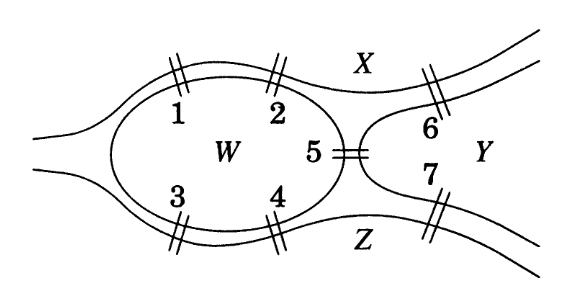
\includegraphics[width=0.5\textwidth]{bridge.jpg}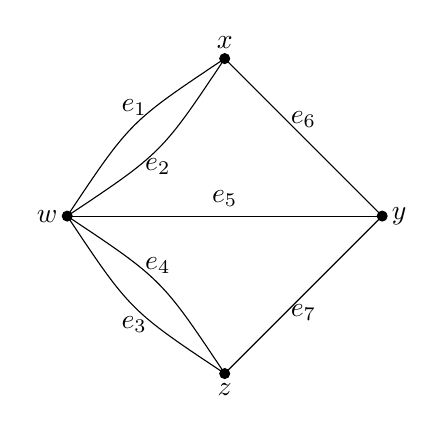
\begin{tikzpicture}
\draw(-2,0)node[left]{$w$}..controls(-1.2,1.2)..node[above]{$e_1$}(0,2);
\draw(-2,0)..controls(-0.8,0.8)..node[below]{$e_2$}(0,2);
\draw(-2,0)..controls(-1.2,-1.2)..node[below]{$e_3$}(0,-2);
\draw(-2,0)..controls(-0.8,-0.8)..node[above]{$e_4$}(0,-2);
\draw(2,0)node[right]{$y$}--node[above]{$e_5$}(-2,0);
\draw(0,2)node[above]{$x$}--node[above]{$e_6$}(2,0);
\draw(0,-2)node[below]{$z$}--node[below]{$e_7$}(2,0);
\fill(-2,0)circle[radius=2pt];
\fill(0,2)circle[radius=2pt];
\fill(2,0)circle[radius=2pt];
\fill(0,-2)circle[radius=2pt];
\end{tikzpicture}\]
The list $x,e_2,w,e_5,y,e_6,x,e_1,w,e_2,x$ forms a closed walk of length 5. Deleting the last edge and vertex yields a trail of length 4. The subgraph consisting of edges $e_1,e_5,e_6$ and vertices $x,y,z$ is a cycle of length 3, and deleting one of the edges yields a path of length 2.
\end{example}

\begin{example}
The \textbf{Petersen graph} is the simple graph with 10 vertices and 15 edges whose vertices are 2-element subsets of $\{1,2,3,4,5\}$ and the edges pair all disjoint such subsets.
\[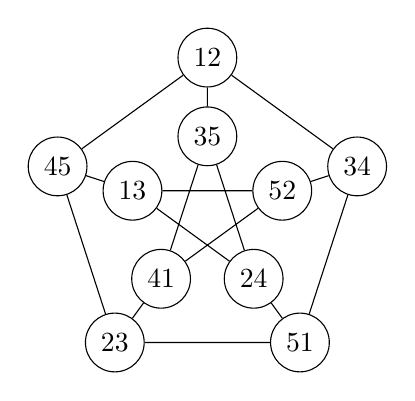
\begin{tikzpicture}
\tikzstyle{every node}=[draw,shape=circle,minimum size=0.5pt];
\node(v1) at (90:2) {$12$};
\node(v2) at (18:2) {$34$};
\node(v3) at (306:2) {$51$};
\node(v4) at (234:2) {$23$};
\node(v5) at (162:2) {$45$};
\node(v6) at (90:1) {$35$};
\node(v7) at (18:1) {$52$};
\node(v8) at (306:1) {$24$};
\node(v9) at (234:1) {$41$};
\node(v10) at (162:1) {$13$};
\draw(v1)--(v2)(v2)--(v3)(v3)--(v4)(v4)--(v5)(v5)--(v1)(v1)--(v6)(v2)--(v7)(v3)--(v8)(v4)--(v9)(v5)--(v10)(v6)--(v8)(v6)--(v9)(v7)--(v9)(v7)--(v10)(v8)--(v10);
\end{tikzpicture}\]
Petersen graph has girth 5 and ten $6$-cycles.
\end{example}

\begin{example}
The \textbf{$k$-dimensional cube} $Q_k$ is the simple graph whose vertices are $k$-tuples drawn from $\{0,1\}$ and whose edges pair $k$-tuples that differ in exactly one entry.
\end{example}
\[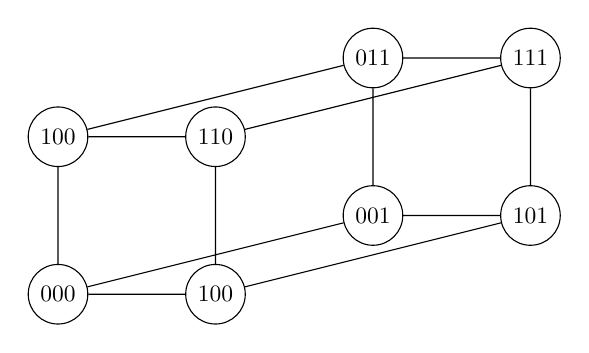
\begin{tikzpicture}
\tikzstyle{every node}=[draw,circle,scale=0.85];
\node(v1) at (-3,1) {$100$};
\node(v2) at (-1,1) {$110$};
\node(v3) at (-3,-1) {$000$};
\node(v4) at (-1,-1) {$100$};
\node(v5) at (1,2) {$011$};
\node(v6) at (1,0) {$001$};
\node(v7) at (3,0) {$101$};
\node(v8) at (3,2) {$111$};
\draw(v1)--(v2)(v2)--(v4)(v4)--(v3)(v3)--(v1)(v1)--(v5)(v2)--(v8)(v3)--(v6)(v4)--(v7)(v5)--(v8)(v8)--(v7)(v7)--(v6)(v6)--(v5);
\end{tikzpicture}\]
$Q_k$ is $k$-regular bipartite graph. Hence it has same number of vertices in each partite sets.



\end{document}